\begin{figure}
	\centering
	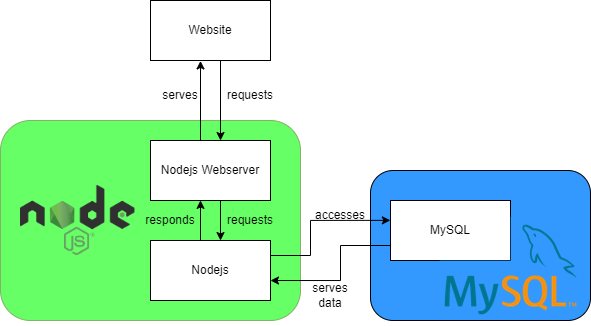
\includegraphics[width=15cm]{images/TechnologyStack.png}
	\caption[Technologiestack]{Technologiestack}
	\label{fig:Technologiestack}
\end{figure}

\subsubsection{Nodejs}
Nodejs ist ein sehr ausgereiftes Framework für Webapplikationen. Es hat eine sehr große Userbase, und ist auch in der Industrie weit verbreitet. Es wird unter anderem von Firmen wie LinkedIn, PayPal und eBay für ihre Internetpräsenz verwendet. Auch die Organisation NASA benutzt Nodejs in ihrem Technologiestack.\cite{nodejs} \newline
In diesem Projekt wird auch der Nodejs interne Webserver verwendet, der obwohl er nicht optimal ist, für den aktuellen Projektstand vollkommen ausreichend.


\subsubsection{MySQL}
Für die Datenspeicherung und das Accountmanagement wird eine Datenbank benötigt. MySQL stellt dafür eine weit verbreitete und einfach zu integrierende Lösung dar. Wie aus dem  Namen hervorgeht ist MySQL eine Datenbank(-sprache) aus der SQL Familie. Die Webanwendungen von Amazon, Twitter, Netflix und Udemy beispielsweise, arbeiten zumindest teilweise mit MySQL. \cite{mysql}

\subsubsection{HTML - Hyper Text Markup Language}
Hyper Text Markup Language oder HTML ist die Programmiersprache mit der Websites geschrieben werden. Das HTML Dokument definiert die generelle Struktur der Seiten und deren Inhalt.

\subsubsection{CSS - Cascading Syle Sheet}
CSS (Cascading Style Sheets) werden genutzt um HTML Dokumente in eine ästhetisch ansprechende Form zu bringen. 

\subsubsection{Javascript}
Javascript ist eine Programmiersprache, die verwendet wird um Webapplikationen responsiv zu gestalten. Das heißt Anpassungen am Inhalt der Website in Echtzeit durchzuführen. „As of 2022, 98\% of websites use JavaScript on the client side for webpage behavior, often incorporating third-party libraries.“ \cite{JavaScript}

\subsubsection{EJS - Embedded Javascript Templating}
Wie aus dem Namen hervorgeht ist Embedded Javascript Templating (kurz EJS) eine Form Websites in Templates aufzutrennen, also eine Website in die wichtigen Komponenten zu zerlegen. Dies hilft sowohl mit der Usability und der Recognizeability der Website, als auch mit dem Layouting, da die verschiedenen Routen teilweise oder komplett mit den gleichen Komponenten aufgebaut werden. Manchmal unterscheidet sich lediglich der Inhalt der Routen.

\subsubsection{Bootstrap}
Die in diesem Projekt verwendete Bibliothek Bootstrap ist eine Bibliothek, die sowohl CSS als auch Javascript Funktionalitäten kombiniert um das Design des Frontends zu erleichtern.

